Slovenské nárečia predstavujú dorozumievací prostriedok autochtónneho obyvateľstva príslušných nárečových oblastí v~každodennom spoločenskom a~pracovnom styku s~najbližším okolím. Slovenské nárečia sa doteraz dedia z~generácie na generáciu v~ústnej podobe, hoci aj tu dochádza v~porovnaní s~minulosťou k~procesu nivelizácie.

Slovnú zásobu jednotlivých nárečí na území Slovenska opisuje Slovník slovenských nárečí, podrobnejšie a~v~rozšírení na ďalšie jazykové roviny sú viaceré nárečia opísané v~samostatných monografiách.

\begin{figure}[H]
\centering
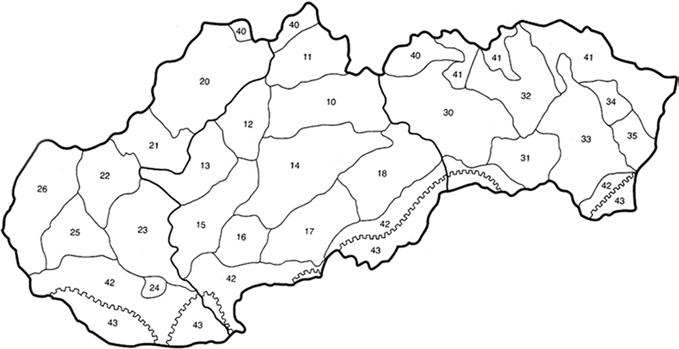
\includegraphics[width=\textwidth]{dialects-map.png}
\caption{%
Mapa slovenských nárečí
}
\label{picture:dialects}
\end{figure}

Slovenské nárečia sa členia na tri základné skupiny:

\begin{itemize}
\item[\bf a)] \textbf{západoslovenské nárečia}

Západoslovenské nárečia sú rozšírené v~trenčianskej, nitrianskej, trnavskej, myjavskej oblasti a~v~ďalších regiónoch.
\begin{enumerate}
\setcounter{enumi}{19}
\item Hornotrenčianske nárečia
\item Dolnotrenčianske nárečie
\item Považské nárečie 
\item Stredonitrianske nárečia 
\item Dolnonitrianske nárečia 
\item Nárečia trnavského okolia
\item Záhorské nárečia 
\end{enumerate}
\item[\bf b)] \textbf{stredoslovenské nárečia}

Stredoslovenskými nárečiami sa hovorí v~regiónoch Liptov, Orava, Turiec, Tekov, Hont, Novohrad, Gemer a~vo~zvolenskej oblasti.
\begin{enumerate}
\setcounter{enumi}{9}
\item Liptovské nárečia
\item Oravské nárečia
\item Turčianske nárečie
\item Hornonitrianske nárečia
\item Zvolenské nárečia
\item Tekovské nárečia
\item Hontianske nárečie
\item Novohradské nárečia
\item Gemerské nárečia
\end{enumerate}
\item[\bf c)] \textbf{východoslovenské nárečia}

Východoslovenské možno nájsť v~regiónoch Spiš, Šariš, Zemplín a~Abov.
\begin{enumerate}
\setcounter{enumi}{29}
\item Spišské nárečia
\item Abovské nárečia
\item Šarišské nárečia
\item Zemplínske nárečia
\item Sotácke nárečia
\item Užské nárečia
\item Oblasť goralských nárečí
\item Oblasť ukrajinských nárečí
\item Nárečovo rôznorodé oblasti 
\item Oblasť maďarských nárečí
\end{enumerate}
\end{itemize}

Tieto skupiny sa ďalej bohato a~pestro členia („Čo dedina, to reč iná“), pričom členitosťou sa nárečia vyznačujú predovšetkým v~hornatých oblastiach. Práve hornatosť krajiny spôsobovala v~minulosti istú (rečovú) izolovanosť obyvateľstva v~rámci jednotlivých žúp. Pod tieto špecifiká sa podpísalo ďalej aj prevrstvovanie a~migrácia obyvateľstva, kolonizácie, miešanie odlišných nárečových typov, pôsobenie susedných slovanských i~neslovanských jazykov, zmeny v~zamestnaní obyvateľstva a~pod. Podľa povahy nárečí a~výskytu jednotlivých charakteristických javov možno zaradiť do uvedených skupín aj slovenské nárečia v~Maďarsku, Srbsku, Chorvátsku, Rumunsku, Bulharsku a~v~iných krajinách, kam sa v~minulosti presídlili veľké kompaktné skupiny. Pri menšom počte starých písomných pamiatok sú slovenské nárečia základným prameňom slovenskej historickej gramatiky.
